\section{Results}

The sweep completed 5{,}520 runs with 28 failures (0.51\%), all one cause:
two cells where no five path edges could be closed without disconnecting the
pair. All stretch invariants hold with zero violations.

\subsection{Extraction provenance decides what a Physarum number means}
\label{sec:cprov}

Pooled across extraction methods, Physarum matches the optimal route on
\textbf{90.0\%} of undisrupted pairs at heavy demand and 86.7\% at light,
reproducing the accuracy this model is credited with. Restricted to its own
maximum-flux walk, the same solves give \textbf{23.3\% and 16.7\%}. The walk
produces any path at all on 69.8\% of Physarum rows.

\begin{table}[t]
\caption{Provenance of Physarum's reported path (776 successful rows). The
median stretch is 1.000 in \emph{every} class.}
\label{tab:cprov}
\centering
\begin{tabular}{lrrrr}
\toprule
Extraction method & Own? & $n$ & Share & Exact \\
\midrule
\texttt{full\_graph\_fallback}     & no  & 315 & 40.6\% & 95.2\% \\
\texttt{max\_flux\_walk}           & yes & 232 & 29.9\% & 74.6\% \\
\texttt{theta\_subgraph\_fallback} & no  & 229 & 29.5\% & 94.3\% \\
\bottomrule
\end{tabular}
\end{table}

About \textbf{70\% of reported Physarum paths did not come from its own
extraction}, and \texttt{full\_graph\_fallback} is plain Dijkstra. Since the
median stretch is exactly 1.000 within each class
(Table~\ref{tab:cprov}), a pooled median cannot separate ``the model found
the optimum'' from ``the fallback returned Dijkstra's answer'', and a pooled
Physarum-versus-Dijkstra comparison is partly circular.

On recovery the effect is sharper and \emph{mode-dependent}. Cold start
splits walk/threshold/full-graph as 95/201/62 (17.3\% Dijkstra); warm start
as 119/\textbf{0}/\textbf{239}. With roughly 98.8\% of retained tubes below
$\theta$, warm's threshold subgraph never connects the pair, a hard zero across all
358 cells, so \textbf{warm Physarum reports plain Dijkstra's
path on two-thirds of recoveries}.

Fig.~\ref{fig:cconv} is the clearest evidence: in two of three panels the
with-fallback curve sits at stretch 1.0 from iteration one, because it was
Dijkstra's answer before the model did any work. We therefore report
Physarum as two labelled series throughout and never pool them.

\begin{figure*}[t]
\centering
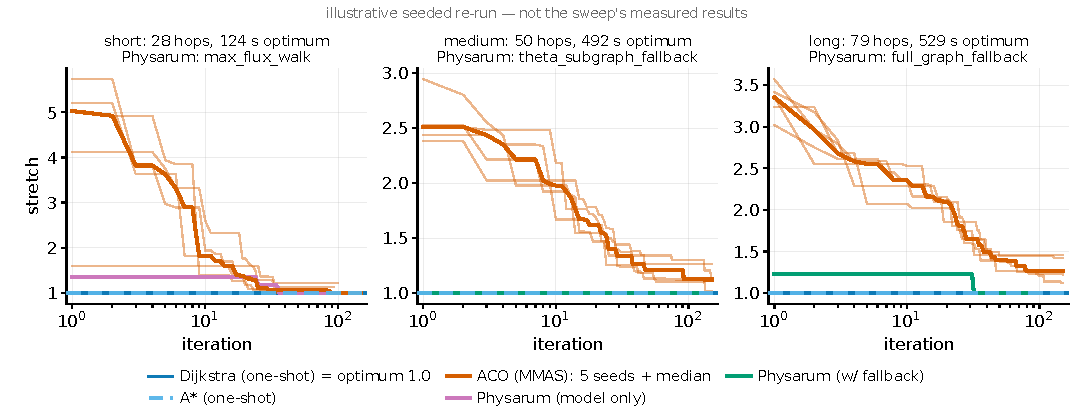
\includegraphics[width=\figw]{fig01_convergence.pdf}
\caption{Cost versus iteration across three distance strata. The Physarum
with-fallback series starts at stretch 1.0 in two of three panels: that is
the fallback, not convergence.}
\label{fig:cconv}
\end{figure*}

For context, ACO reaches 43.3\%/44.0\% exact match with median stretch
1.0052 (light) and 1.0209 (heavy), and Dijkstra and A* are exact by
construction. ACO \emph{misses} the exit criterion we set in advance
(stretch $\leq 1.10$ on $\geq 90\%$ of pairs), reaching 73.3\% under free
flow with a 95\% CI of [58.7, 86.7] entirely below the bar; the failure mode
is a colony settling on a wrong corridor, with MMAS's own convergence
criterion firing on most such solves. We report this rather than retuning
until it passes.

\subsection{Warm start buys speed and charges quality}

\begin{table}[t]
\caption{Recovery cost, scenarios S1--S6. Dijkstra is the honest baseline:
no method here approaches it on wall-clock.}
\label{tab:crecovery}
\centering
\small
\begin{tabular}{llrrrr}
\toprule
Algorithm & Start & $n$ & Iters & Wall (s) & 1 iter \\
\midrule
Dijkstra  & cold & 358 & 1.0 & 0.031 & 100\% \\
A*        & cold & 358 & 1.0 & 0.027 & 100\% \\
ACO       & warm & 1790 & 69.0 & 34.07 & 0\% \\
ACO       & cold & 1790 & 110.0 & 59.80 & 0\% \\
Physarum  & warm & 358 & 42.0 & 0.235 & \textbf{48.3\%} \\
Physarum  & cold & 358 & 98.0 & 5.661 & 0\% \\
\bottomrule
\end{tabular}
\end{table}

Table~\ref{tab:crecovery} gives the raw cost, and the first thing it shows is
that \textbf{Dijkstra wins on wall-clock, which we report rather than hide}: a
recompute on this graph costs about 31\,ms where the bio-inspired methods take
seconds. The defensible quantities are iterations-to-adapt and
post-disruption quality.

Paired on identical cells, warm start cuts Physarum's recovery by
\textbf{2.97$\times$ in iterations} (faster on 350/358,
$p=3.2\times10^{-59}$) and \textbf{6.87$\times$ in wall-clock} (336/358,
$p=9.0\times10^{-52}$); ACO gains 1.26$\times$ and 1.56$\times$
($n=1{,}790$).

Two points matter more than the ratios. The distribution is \textbf{bimodal,
not merely shifted}: 48.3\% of warm recoveries converge in exactly one
iteration while cold start never does and its minimum is 73
(Fig.~\ref{fig:cwc}). The ratio of the two medians is therefore not a valid statistic; an earlier version of this analysis computed one and produced
a spurious 24$\times$. And \textbf{per-iteration cost is essentially
identical} warm versus cold (0.0511 vs 0.0538\,s), establishing that the
saving is fewer iterations rather than cheaper ones.

\begin{figure*}[t]
\centering
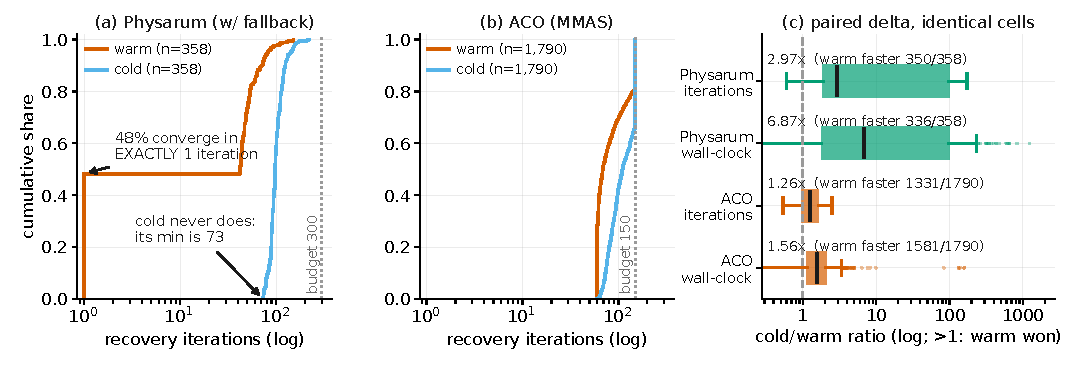
\includegraphics[width=\figw]{fig07_warm_vs_cold.pdf}
\caption{Warm versus cold recovery. The mode at exactly one iteration is the
shape of the result and the reason we report paired ratios.}
\label{fig:cwc}
\end{figure*}

\textbf{The cost.} On the reported path, paired across all 358 cells, cold
start is better: cold wins 57, warm 11, 290 ties
($p=4.3\times10^{-7}$). On the model's own extraction, the warm walk
completes on only 36.3\% of recoveries against cold's 59.5\%. Reporting the
speed-up alone describes half the effect.

\textbf{Why.} We tested the obvious mechanism, a retained field driving flux down severed
corridors, and \emph{refuted} it: a placebo closure at
least eight hops away reproduces nearly the whole deficit and is
indistinguishable from a closure directly on the route (43.3\% vs 41.7\%,
$n=60$ paired, $p=1.00$). A second candidate, that warm start leaves less
conductivity, is \emph{analytically impossible}: scaling $D$ by $c$ scales
$w$ by $c$ and $p$ by $1/c$, leaving $Q=w\Delta p$ unchanged (verified
numerically to $<10^{-15}$). What the data support is that \textbf{the walk
works on a near-uniform field and stops working as the field converges onto
a thin corridor}: convergence alone, with no closure, drops completion from
69.8\% to 43.0\%, and cold start's advantage is that it rewinds the field to
a walkable state.

\begin{figure*}[t]
\centering
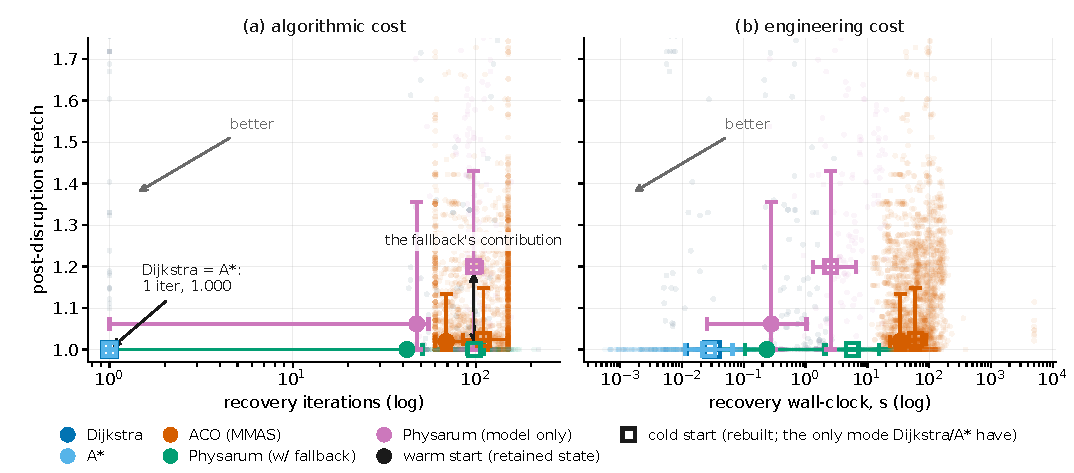
\includegraphics[width=\figw]{fig04_pareto_recovery_vs_quality.pdf}
\caption{The speed-versus-quality trade. Markers are medians with IQR arms
over the individual S1--S6 recovery runs; Dijkstra and A* anchor the lower
left. The model-only and pooled Physarum series share the same runs, so
\emph{the vertical gap between them is the fallback's contribution}.}
\label{fig:cpareto}
\end{figure*}

\subsection{What adaptation contributes}

This invites the conclusion that the model should stop earlier. Against a zero-adaptation control (the same pressure solve on a uniform
field, containing none of the Tero dynamics, and exact by construction since
the solver extracts before updating $D$), the converged field completes
\emph{less} often (0.433 vs 0.567) yet is far better when it does (median
stretch \textbf{1.0059} vs 1.4367; exact given completion 46.2\% vs 5.9\%).
Paired, the unadapted field loses 26--0 to the best adapted iteration
($n=34$, $p=8.3\times10^{-6}$), reproducing at scale on cold recovery
(120--1, $p=3.2\times10^{-21}$).

\textbf{Completion and quality move in opposite directions}, because a
near-uniform field is walkable precisely \emph{because} it is uninformative.
This also resolves the tension with~\cite{wang2021transition}: their claim
concerns quality, which does improve with convergence; what fails here is
completion, which a complete graph cannot exhibit. Consequently \textbf{no
earlier stopping rule is worth adopting}: a perfect per-cell oracle buys
\emph{zero} additional exact matches, since every exact-match walk is
already exact at convergence, and the router already retains the best walk
across iterations.

\subsection{The congestion model decides the sign of the effect}

On the undisrupted solve, ACO's within-10\% rate is 81.3\% under light SUMO
demand and 58.0\% under heavy, and paired on the same (OD, seed) cells heavy
is significantly worse ($p=0.036$; 37 pairs pass only under light against 2
only under heavy).

This \emph{reverses} what we measure on the analytic BPR provider, where
congestion improves ACO's outcomes because it flattens the cost surface so
more routes land within 10\% of optimal. The algorithm, the network and the
OD pairs are identical; only the congestion source differs. SUMO puts signal
delay in the numerator but not the free-flow denominator, while BPR loads
synthetic demand onto shortest paths, which is exactly where an OD-path
measurement walks.

\textbf{So the sign of the congestion effect is a property of the congestion
model, not of the algorithm}, and any claim about routing behaviour ``under
congestion'' that does not name its congestion model is underdetermined. We
accordingly retract a framing from our own earlier analysis, that the two
bio-inspired methods fail in opposite directions under congestion, which held
on BPR and does not survive SUMO, where both degrade.
